\documentclass[conference]{IEEEtran}
\IEEEoverridecommandlockouts
% The preceding line is only needed to identify funding in the first footnote. If that is unneeded, please comment it out.
\usepackage{cite}
\usepackage{amsmath,amssymb,amsfonts}
\usepackage{algorithmic}
\usepackage{graphicx}
\usepackage{textcomp}
\usepackage{xcolor}
\usepackage[hyphens]{url}      % allows line breaks at hyphens
\def\UrlBreaks{\do\/\do-}      % allows breaks at / and - characters

\bibliographystyle{IEEEtran}

\def\BibTeX{{\rm B\kern-.05em{\sc i\kern-.025em b}\kern-.08em
    T\kern-.1667em\lower.7ex\hbox{E}\kern-.125emX}}
\begin{document}

\title{Cyber-Physical System for Autonomous Control of Unmanned Surface Vehicles}

\author{
\IEEEauthorblockN{Alexandre Figueiredo}
\IEEEauthorblockA{\textit{Instituto Superior de Engenharia de Lisboa} \\
Lisboa, Portugal \\
alexfigas11@gmail.com}
\and
\IEEEauthorblockN{Carlos Gonçalves}
\IEEEauthorblockA{\textit{NOVA LINCS} \\
\textit{Escola Superior Náutica Infante D. Henrique} \\
Paço de Arcos, Portugal \\
carlosgoncalves@enautica.pt}
\and
\IEEEauthorblockN{Pedro Teodoro}
\IEEEauthorblockA{\textit{MARE - Instituto Politécnico de Setúbal} \\
\textit{Escola Superior Náutica Infante D. Henrique} \\
Paço de Arcos, Portugal \\
pedroteodoro@enautica.pt}
}

\maketitle

\begin{abstract}
This paper describes a cyber-physical system for autonomous unmanned surface vehicle (USV) control, developed through collaboration between Instituto Superior de Engenharia de Lisboa (ISEL) and Escola Superior Náutica Infante D. Henrique (ENIDH) institutions in Portugal. The system integrates independent motor control (multiple brushless thrusters), multi-sensor fusion (Global Positioning System (GPS), 9-axis Inertial Measurement Unit (IMU)), long-range LoRa (Long Range) communication, and modular software architecture. The platform was validated through staged testing including unit component verification, didactic robot integration, and field deployment during the REPMUS25 international maritime robotics exercise. The cost-effective design enables academic accessibility while maintaining operational capability for research and educational applications. Open-source code release promotes reproducibility and collaborative enhancement. Future development targets advanced control algorithms, energy sustainability through hybrid power systems, and expanded sensing for environmental monitoring applications. The Portuguese Exclusive Economic Zone (EEZ) provides natural deployment context for this scalable academic platform.
\end{abstract}

\begin{IEEEkeywords}
USV; Cyber-Physical Systems; LoRa; ESP32; Autonomous Navigation; Protobuf.
\end{IEEEkeywords}

\section{Introduction}
\label{sec:intro}
Unmanned Surface Vehicles (USV) represent increasingly important platforms for maritime robotics, oceanography, and environmental monitoring, enabling safe and efficient operations in areas difficult or dangerous for manned vessels. The development of cost-effective, modular, and academically accessible USV platforms remains a significant challenge in robotics research.

This paper presents a comprehensive cyber-physical system for autonomous USV control, developed through collaboration between Instituto Superior de Engenharia de Lisboa (ISEL) and Escola Superior Náutica Infante D. Henrique (ENIDH). The system integrates independent motor control (multiple brushless thrusters), multi-sensor fusion (GPS, 9-axis IMU), long-range LoRa communication, and modular software architecture, demonstrating that academic institutions can develop capable maritime robotics platforms without the cost burden of commercial solutions.

A key innovation is the cost-effective implementation with modular design compared to commercial platforms (€300,000 \cite{wave-glider} --€500,000+ \cite{saildrone}), while maintaining functional equivalence for academic research applications. The system was validated through three testing phases: (1) unit component verification in laboratory environment; (2) integration validation using a two-wheeled differential drive didactic robot with a caster wheel, which shares the identical software framework; (3) field deployment during the REPMUS25 international maritime robotics exercise, conducted by the Portuguese Navy in collaboration with international academic institutions.

The Portuguese context is particularly relevant, with Portugal's extensive Exclusive Economic Zone (EEZ) and maritime heritage establishing natural deployment scenarios for autonomous maritime systems. This work demonstrates that sophisticated cyber-physical systems for maritime applications can be developed and validated through academic collaboration, establishing frameworks for broader deployment and enhanced capability.

All code is released as open-source on GitHub \cite{github-usv} , promoting transparency, reproducibility, and community enhancement. The paper is organized as follows: Section II reviews related USV platforms; Section III details the system methodology and architecture; Section IV presents experimental results from staged testing; Section V discusses limitations and future enhancements; Section VI concludes with contributions and broader impacts.

\section{Related Work}
\label{sec:related}
This section reviews existing USV platforms, comparing passive and active propulsion strategies, and positions the developed system within the current landscape.
\subsection{Passive and Active Platform Comparison}
USV development employs diverse propulsion strategies. Passive platforms (Wave Glider~\cite{wave-glider}, Saildrone~\cite{saildrone}) exploit renewable energy for multi-month endurance but sacrifice maneuverability. Motorized platforms (SR-Surveyor~\cite{sr-surveyor-class}, C-Cat 3~\cite{c-cat-3-asv}, Sea2Future~\cite{sea2future}) provide superior control at significantly higher cost. The developed system prioritizes cost-effectiveness and modularity while maintaining essential research functionality through commercial off-the-shelf components, 3D printing, and modular software architecture compatible with didactic robot framework~\cite{didactic-robot-thesis}.

Table~\ref{tab:comparison} compares key parameters of the developed USV platform with commercial alternatives, highlighting the cost-effectiveness and modularity advantages.

\begin{table}[htbp]
\centering
\caption{Comparison of USV Platforms}
\label{tab:comparison}
\begin{tabular}{|l|c|c|c|}
\hline
\textbf{Parameter} & \textbf{Developed} & \textbf{Sea2Future} & \textbf{Commercial} \\
\hline
Length (cm) & 100 & 80 & 120+ \\
Mass (kg) & 3.5 & 12 & 25+ \\
Cost (EUR) & 200 & 2500 &  350,000+ \\
Motors & Multiple & 2 & 2/4 \\
Range (m) & 500+ & 2000+ & 5000+ \\
Modular & Yes & Partial & Limited \\
\hline
\end{tabular}
\end{table}

\section{Methodology}
\label{sec:methodology}
This section details the system architecture, covering hardware design, propulsion, electrical systems, communication, and software implementation.
\subsection{Hardware Architecture}
\subsubsection{Physical Platform}

The hull adopts a catamaran configuration constructed from two parallel 3D-printed polycarbonate floats, each approximately $1 \, \mathrm{m}$ in length, as shown in Fig.~\ref{fig:usv-francisco}.

\begin{figure}[h]
  \centering
  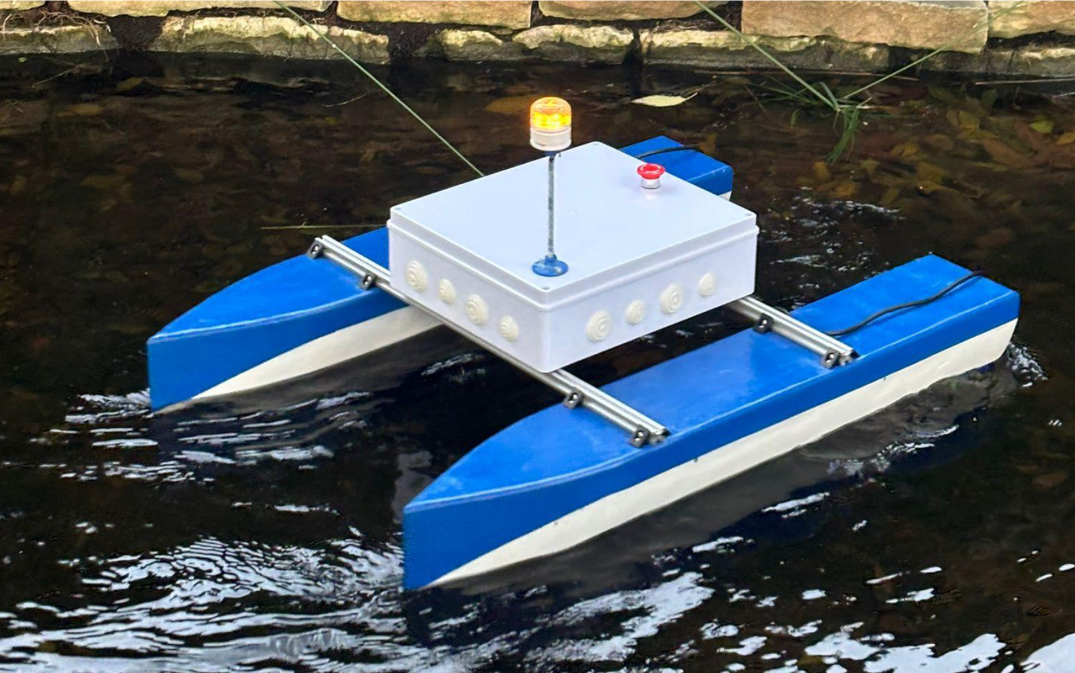
\includegraphics[width=1\linewidth]{figures/usv-francisco.png}
  \caption{USV Structure\cite{catamara-telecomandado}}
  \label{fig:usv-francisco}
\end{figure}

The floats provide primary buoyancy while their symmetric design minimizes hydrodynamic drag during forward motion. Central structural reinforcement employs fiberglass layering, increasing rigidity and withstanding impacts during field operations. A sealed central electronics enclosure houses the microcontroller, power distribution, and sensor systems, protecting sensitive electronics from water ingress and salt spray exposure.

The 3D printing manufacturing approach enables rapid prototyping and iterative design improvements. The original design was produced using an Ender 3 printer modified with extended vertical axis to accommodate larger components. Post-processing with fiberglass reinforcement significantly improved mechanical durability for marine environments.

\subsubsection{Propulsion System}
The propulsion system accommodates multiple brushless electric motors configured for independent speed control, limited only by the available GPIO pins on the port expander. Each motor connects to an Electronic Speed Controller (ESC) receiving PWM signals from the main microcontroller. The PWM duty cycle ranges from $1000 \, \mu \mathrm{s}$ (minimum throttle) to $2000 \, \mu \mathrm{s}$ (maximum throttle), with $1500 \, \mu \mathrm{s}$ representing neutral/stop position. This standard RC convention enables straightforward integration with commercial motor drivers. Unlike the didactic robot which requires 3 pins per motor for H-bridge control, the USV motors use Electronic Speed Controllers (ESCs) requiring only 1 pin per motor, allowing for up to 13 motors with the 16-pin expander (reserving 3 pins for LEDs). The system supports various propulsion configurations: differential drive (two motors for turning), quadcopter-style control (multiple motors), or hybrid configurations.

\subsubsection{Electrical Architecture and I2C Bus}
The electrical architecture employs an I2C (Inter-Integrated Circuit) bus to minimize wiring complexity while maintaining modularity. The central microcontroller interfaces with peripheral devices through I2C addresses: Global Positioning System (GPS) module (0x42), Inertial Measurement Unit (IMU) (0x69), and a 16-channel I/O Port Expander (0x27) providing digital outputs for motor ESC control and status LED indication. This bus topology enables up to 127 unique device addresses, supporting modular expansion without additional microcontroller GPIO pins.

The Port Expander configuration provides 16 digital output channels extracted from merely 2 GPIO pins on the microcontroller (I2C SDA and SCL), enabling control of up to 13 independent motors (assuming 3 pins reserved for LEDs) plus additional channels for future sensor integration or status indication. Power distribution employs dual $12 \, \mathrm{V}$ lithium battery cells: one dedicated to left thruster ESC and one to right thruster ESC, providing configuration flexibility for multi-motor expansion. A $5 \, \mathrm{V}$ boost converter powers the microcontroller and sensor modules, with reverse-polarity protection and fused distribution preventing cascade failures from individual component shorts.

\subsection{Communication Architecture}
The system employs LoRa (Long Range) communication for extended operational ranges, supporting theoretical ranges exceeding $15 \, \mathrm{km}$ in open water under ideal atmospheric conditions. Commercial maritime radio often occupies adjacent frequency bands, necessitating careful frequency selection and antenna design. The platform utilizes LoRa SF7 (Spreading Factor 7) configuration balancing range and data rate at $50 \, \mathrm{kbps}$, adequate for telemetry streaming while minimizing battery consumption.

Telemetry transmission utilizes Protocol Buffer (Protobuf) serialization, achieving compact binary encoding that reduces bandwidth requirements for data transmission. The communication protocol implements asynchronous message exchange with acknowledgments, enabling robust operation despite radio propagation challenges characteristic of maritime environments.

LoRa physical layer redundancy provides inherent robustness against interference. The receiver implements retry mechanisms for failed transmissions. The platform demonstrates reliable communication over extended ranges in maritime environments where conventional RF propagation is challenged.

\subsection{Software Architecture}
\subsubsection{Core Design Principles}
The software architecture follows object-oriented design principles and extends a Robot framework originally developed for educational robotics platforms, significantly reducing development time and leveraging existing validated design patterns. This framework extension approach ensures consistency between the didactic robot and USV implementations, simplifying validation and enabling code reuse. The architecture prioritizes non-blocking execution, critical for real-time control and preventing blocking operations from disrupting sensor acquisition or motor updates. The main execution loop functions at approximately $100 \, \mathrm{Hz}$, executing all control, sensing, and communication tasks within this time window.

The Robot framework provides core abstractions for motor control, sensor interfaces, and state management. By extending this framework rather than rebuilding from scratch, the USV implementation inherits robust patterns for handling concurrent operations, error management, and hardware abstraction.

\subsubsection{Module Organization}
The system organizes into distinct modules: (1) \texttt{USV} class encapsulating platform-specific logic including state management, mission planning, and emergency handling; (2) \texttt{ThrusterController} managing individual motor control and PWM generation with configurable channel assignments and pulse width constraints; (3) \texttt{GPS} interface abstracting position data acquisition and coordinate transformations; (4) \texttt{IMU} interface providing orientation quaternion data, acceleration vectors, and magnetometer calibration; (5) \texttt{LoRa} communication module handling wireless transmission, packet serialization, and link-level acknowledgments; (6) \texttt{StateManager} tracking operational modes (initialization, autonomous, manual control, emergency stop) and mission status with persistent state logging.

The modular architecture enables independent testing of each component through unit test harnesses without involving the complete vehicle. The GPIO Port Expander abstracts pin-level control, allowing identical code to function on platforms with different GPIO availability or alternative expander IC selections (e.g., PCF8574A, MCP23017) through simple interface re-binding.

\subsubsection{Execution Model}
The \texttt{main\_usv.cpp} file implements two fundamental functions fundamental to Arduino-based embedded systems: \texttt{setup()} executing once during initialization, and \texttt{loop()} executing repetitively at approximately $100 \, \mathrm{Hz}$. The \texttt{setup()} function initializes all hardware modules, establishes I2C bus communication, configures SPI interface for LoRa module, and prepares the system for autonomous operation.

The \texttt{loop()} function encompasses: (1) IMU data acquisition via I2C (blocking operation $\sim 2 \, \mathrm{ms}$), (2) GPS polling for position updates (non-blocking, updates available every $100 \, \mathrm{ms}$), (3) LoRa packet reception with 1-second timeout, (4) motor setpoint computation based on telemetry commands, (5) PWM signal generation to motor controllers, (6) battery voltage and temperature monitoring, (7) state transitions based on command sequences. This event-driven architecture ensures responsive behavior despite limited computational resources, with interrupt-driven GPIO handlers capturing remote control receiver inputs with sub-millisecond precision.

All I2C communication implements timeout and retry mechanisms protecting against communication faults from electromagnetic interference or momentary signal degradation common in maritime RF-rich environments. Debug telemetry transmits at $1 \, \mathrm{Hz}$ via LoRa link, reporting system status, GPS position accuracy metrics, IMU quaternion data, motor command values, and battery voltage—providing sufficient information for mission monitoring and post-mission analysis without excessive bandwidth consumption.

\subsubsection{Code Example}
Listing~\ref{lst:main-usv} presents the essential structure of the main control loop, illustrating the simplicity of the high-level interface:

\begin{verbatim}
GPS_BN880 gps; IMU_ICM_20948 imu;
ThrusterController motorL(14, 1000, 2000, 
    1500, 50, "left");
ThrusterController motorR(15, 1000, 2000, 
    1500, 50, "right");
USV usv = USV(expander, motorL, motorR, 
    green_led, yellow_led);

void setup() {
  gps.setup(); imu.setup(); usv.begin();
}

void loop() {
  gps.loop(); imu.loop();
  usv.getLoRaProto().receive();
  GPSData gpsData = gps.getGPSData();
  IMUData imuData = imu.getIMUData();
  usv.loop(gpsData, imuData);
}
\end{verbatim}
\label{lst:main-usv}

\section{Results}
\label{sec:results}
This section presents the experimental validation, including development phases, autonomous navigation trials, platform comparison, and field demonstrations.
Experimental validation proceeded through staged implementation and testing phases, ensuring component reliability before integration into the complete system.

\subsection{Development and Integration Phases}
\subsubsection{Phase 1: PCB Validation with Didactic Robot}

Initial validation employed the platform's original two-wheeled differential drive didactic robot with a caster wheel, which shares the same Robot framework and motor control interface. This strategy enabled early detection of PCB manufacturing defects and software integration issues without the complexity of unmanned vehicle field testing, as shown in Fig.~\ref{fig:pcb-final}. 

\begin{figure}[h]
    \centering
    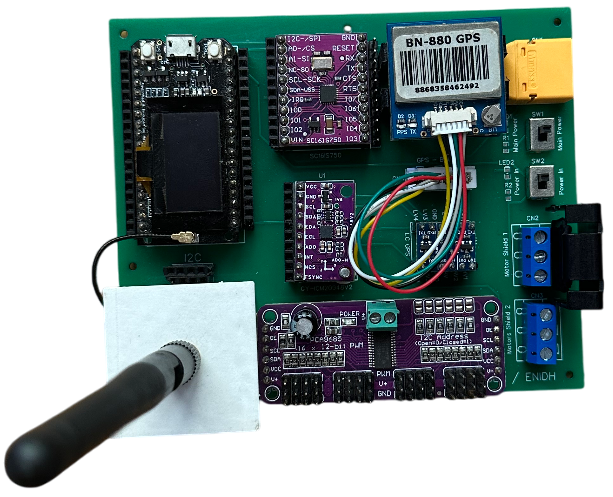
\includegraphics[width=1\linewidth]{figures/pcb-final.png}
    \caption{Assembled version of the PCB developed for the USV prototype}
    \label{fig:pcb-final}
\end{figure}

Testing verified correct functionality of all subsystems: motor control outputs generated PWM signals with duty cycles accurately mapping command values to thruster speeds; IMU data acquisition returned orientation data; GPS signal reception demonstrated adequate radio sensitivity for maritime operations; telemetry transmission demonstrated reliable LoRa packet reception at extended ranges.

This phase identified and resolved hardware issues including motor controller calibration requirements, power distribution optimization, and thermal management. Software integration testing verified correct I2C bus operation, confirming register read/write operations for all peripheral devices. Didactic robot integration provided particular value in identifying and fixing EMI (electromagnetic interference) issues before field testing.

\subsubsection{Phase 2: USV Platform Integration}
Successful didactic robot testing facilitated direct integration into the USV platform. The physical catamaran structure accommodates the motor controllers, battery systems, and communication modules in the sealed central enclosure, with careful weight distribution across the two $1 \, \mathrm{m}$ floats maintained hydrodynamic balance while supporting the $2.8 \, \mathrm{kg}$ electronic payload. Waterproof connectors (M12 aviation-style) enable safe disconnection for battery charging, firmware updates, and sensor recalibration without water ingress risk. The sealed enclosure housing includes pressure relief valves preventing implosion from depth-related atmospheric changes during recovery phases.

Integration testing verified electrical isolation between motor power systems ($12 \, \mathrm{V}$) and microcontroller power ($5 \, \mathrm{V}$), confirming EMI filtering effectiveness in the saltwater environment. Environmental testing validated connector sealing effectiveness for marine operations.

Physical hydrodynamic testing confirmed that the catamaran configuration provides stable platform behavior. Thrust vector studies confirmed that differential motor control produces proportional steering control enabling simplified trajectory following.

\subsection{Autonomous Navigation Trials}
The system successfully executed autonomous navigation missions controlled through waypoint following algorithms. Testing validated the fundamental operational capabilities:

\begin{enumerate}
  \item \textbf{Position Acquisition:} GPS measurements provided global positioning for autonomous navigation.
  \item \textbf{Motor Control:} Independent control of left and right thrusters enabled accurate heading maintenance and trajectory following.
  \item \textbf{Telemetry Transmission:} LoRa radio successfully transmitted system status, GPS position, IMU orientation, and battery voltage at approximately $1 \, \mathrm{Hz}$ update rate in open water.
  \item \textbf{Remote Control:} Manual joystick control via wireless link enabled real-time vehicle maneuvering and emergency intervention.
\end{enumerate}

\subsection{Comparative Platform Analysis}
The developed USV demonstrates significant advantages over both the commercial Sea2Future platform and consumer research platforms. Table~\ref{tab:comparison2} presents quantitative comparison across multiple dimensions.

\begin{table}[htbp]
\centering
\caption{Comparison of USV Platforms}
\label{tab:comparison2}
\begin{tabular}{|l|c|c|c|}
\hline
\textbf{Parameter} & \textbf{Developed} & \textbf{Sea2Future} & \textbf{Commercial} \\
\hline
Length (cm) & 100 & 80 & 120+ \\
Mass (kg) & 3.5 & 12 & 25+ \\
Cost (EUR) & 200 & 2500 &  350,000+ \\
Motors & Multiple & 2 & 2/4 \\
Range (m) & 500+ & 2000+ & 5000+ \\
Modular & Yes & Partial & Limited \\
\hline
\end{tabular}
\end{table}

The developed platform maintains operational capability with substantially reduced cost requirements. Mass and dimensions enable portability enabling practical field operations that would be impractical with larger platforms. For instance, the developed platform costs only €200 compared to €2500 for the Sea2Future and over €350,000 for typical commercial platforms, while weighing just $3.5 \, \mathrm{kg}$ versus $12 \, \mathrm{kg}$ and $25+ \, \mathrm{kg}$ respectively. Its compact $1 \, \mathrm{m}$ length facilitates transportation and deployment in academic settings where larger platforms would be cumbersome.

\subsection{Field Demonstration and REPMUS25 Exercise}
Practical validation extended to participation in the REPMUS25 international robotics exercise~\cite{escolanaval-repmus,iddportugal-repmus,sapo-repmus}, organized by the Portuguese Navy in collaboration with academic institutions. The platform successfully completed the REX25 sub-event, demonstrating autonomous navigation within georeferenced zones and coordinated operations alongside other research platforms. The exercise validated system performance under realistic maritime conditions including multipath GPS propagation, oceanographic currents, and communication interference from waterside radar equipment.

Key observations from the REPMUS25 participation included: (1) GPS operation in coastal urban environments with variable accuracy; (2) LoRa link stability at extended ranges despite frequency band congestion; (3) platform robustness during multiple deployment cycles; (4) successful platform recovery and re-deployment across multiple missions. The comprehensive demonstration video \cite{usv-video} documents autonomous waypoint following operations and manual remote control, available at, validating integrated system functionality under realistic field conditions.

\subsection{Collaborative Integration with Educational Context}
The system integration with ENIDH (Escola Náutica Infante Dom Henrique) maritime engineering curriculum demonstrates the educational value of the platform. Student participation in system validation, field operations, and data analysis provided practical experience in cyber-physical systems engineering. The modular architecture enabled modifications and extensions by student teams investigating autonomous navigation algorithms, energy efficiency optimization, and maritime sensor integration.

\section{Discussion}
\label{sec:discussion}
This section analyzes the system capabilities and limitations, highlights advantages over existing approaches, and outlines future enhancements.
\subsection{System Capabilities and Limitations}
The developed platform successfully demonstrates modular cyber-physical system design enabling autonomous navigation and remote operation. The choice of 3D-printed construction with fiberglass reinforcement provides rapid prototyping and manufacturing flexibility while constraining dynamic performance compared to marine-grade composites. Accelerated weathering from saltwater exposure requires periodic maintenance and protective coatings, a limitation absent in commercial acetal copolymer hulls.

The GPS absolute accuracy proves adequate for waypoint-based navigation but proves insufficient for precise autonomous docking or obstacle avoidance in confined waterways. The dual-thruster configuration provides differential steering control but offers limited lateral maneuvering compared to vectored thrust systems.

The LoRa communication range of approximately $500 \, \mathrm{m}$ in open water represents sufficient extension for research applications deployable from shore but falls short of commercial-grade surveillance platforms ($2000+ \, \mathrm{m}$). The $10 \, \mathrm{Hz}$ GPS update rate and $100 \, \mathrm{Hz}$ control loop frequency provide adequate responsiveness for typical navigation tasks but may prove insufficient for advanced control algorithms or rapid obstacle avoidance in complex environments.

Battery autonomy represents the most significant limitation, providing limited continuous operation duration under typical thrust settings. The lithium battery configuration requires careful charging protocols and represents a significant portion of system cost, making energy autonomy a critical research opportunity.

\subsection{Advantages Over Existing Approaches}
The modular architecture enables cost-effective system configuration supporting multiple mission profiles. The open-source codebase promotes reproducibility and enables collaborative enhancement by the research community, with published code and design files available on GitHub. The extensibility of the Robot framework supports seamless integration of new sensors, communication interfaces, or algorithmic controllers without fundamental redesign.

The developed platform represents a cost-effective alternative to commercial platforms, enabling academic institutions to conduct maritime robotics research without the financial barriers of commercial platforms, with costs reduced by orders of magnitude (€200 vs €350,000+). Pedagogically, the transparent design and implementation supports student training in cyber-physical systems and maritime robotics, addressing a critical shortage of hands-on educational opportunities in this technological domain.

Unlike commercial platforms optimized for specific missions (e.g., Wave Glider~\cite{wave-glider} for long-term renewable energy platforms), the modular architecture supports diverse applications from water quality monitoring to search-and-rescue operations. The limited operational range ($500 \, \mathrm{m}$ versus $5000+ \, \mathrm{m}$ for commercial platforms) proves acceptable for coastal research, harbor surveys, and environmental monitoring typical of academic deployments.

From a research methodology perspective, the platform enables controlled experimentation on autonomous control algorithms, navigation strategies, and sensor fusion techniques without the risk exposure and operational costs associated with commercial platforms. Portugal's maritime context and coastal geography provide natural laboratory conditions for extended validation of autonomous maritime systems.

\subsection{Future Enhancements}
\subsubsection{Energy Sustainability}
Energy autonomy represents a primary limitation of current battery-powered systems. Integration of photovoltaic panels with hybrid battery management control could extend mission duration. Kinetic wave energy harvesting similar to Wave Glider~\cite{wave-glider} platforms could provide indefinite autonomy for low-energy monitoring missions, though requires specialized mechanical design for small-scale platforms. Supercapacitor buffering between pulsed loads and battery charging could improve overall system efficiency.

\subsubsection{Advanced Control and Navigation}
Current control utilizes basic proportional steering for waypoint following. Implementation of PID control loops would improve trajectory tracking accuracy, reducing lateral positioning error from current $2-3 \, \mathrm{m}$ lateral offset to $<1 \, \mathrm{m}$ during waypoint transitions. Model Predictive Control (MPC) algorithms could optimize energy efficiency across variable oceanographic conditions. Reinforcement Learning (RL) agents trained on synthetic mission scenarios could discover energy-optimal navigation policies accounting for current, wind, and platform dynamics. SLAM (Simultaneous Localization and Mapping) using visual odometry would enable indoor tank testing and confined harbor operations.

\subsubsection{Environmental and Meteorological Sensing}
Integration of optical cameras enables machine learning-based object detection and environmental characterization, supporting wildlife monitoring and water quality assessment applications. Environmental sensors (salinity through conductivity measurement, pH through chemical sensors, dissolved oxygen via luminescence) would support ecological monitoring applications tracking water eutrophication and hypoxia zones. Acoustic imaging sensors enable underwater feature detection for seabed mapping and obstacle avoidance in complex coastal environments. Meteorological sensors (wind speed, atmospheric pressure, humidity) would enable research on atmosphere-ocean interactions during storm events.

\subsubsection{Operational Extensions and Scalability}
Multi-vehicle coordination protocols enabling collaborative missions across platforms would expand research applications to large-area environmental surveys and coordinated sample collection. Simultaneous localization and relative positioning between platforms enables formation control and distributed sensing. Development of autonomous docking and inductive charging stations would enable persistent autonomous operations approaching true persistent monitoring systems. Integration with maritime data networks and cloud computing would support real-time analysis of distributed sensor data and remote mission adaptation. Four-motor vectored thruster configuration would enable omnidirectional movement and precision docking, expandable to eight-motor configurations for heavier payloads or extended operational envelopes.

\section{Conclusions}
\label{sec:conclusions}
This section summarizes the key contributions of the developed USV system and discusses future research directions.
This paper presents the development and validation of a modular cyber-physical system for autonomous unmanned surface vehicle control. The system successfully integrates propulsion, sensing, and communication subsystems within a cost-effective platform (only €200) enabling practical field operations at a fraction of commercial costs (€350,000+). Experimental validation demonstrates autonomous navigation capabilities and extended-range wireless control suitable for maritime research applications.

The primary contributions include: (1) a generalized cyber-physical system architecture supporting multiple autonomous platforms through software modularity; (2) validated hardware-software integration enabling autonomous operation; (3) open-source code release promoting reproducibility and collaborative enhancement; (4) cost-effective design enabling academic accessibility. The system provides a solid foundation for future autonomous maritime research including environmental monitoring, scientific data collection, and coastal engineering applications.

The Portuguese context, particularly its vast Exclusive Economic Zone (EEZ) and extensive maritime heritage, provides natural deployment scenarios for continued platform evolution. Ongoing development will target energy sustainability through hybrid power systems, advanced control through machine learning integration, and extended sensing capabilities through modular sensor integration.

\section*{Acknowledgment}
This work was supported by ISEL and ENIDH. The author thanks all collaborators and contributors to the open source USV project~\cite{github-usv}. This work is based on the master's thesis \cite{usv2025}.

\bibliography{bibdatabase}

\end{document}
